\documentclass[draft]{beamer}
\usetheme{Warsaw}
\usepackage{ifdraft}
\usepackage{standalone}
\usepackage{lmodern} % Allows arbitrary font sizes to prevent warnings.
\usepackage{tikz}
\usetikzlibrary{patterns}
\usetikzlibrary{calc}
\definecolor{printred}{RGB}{215,25,28}
\definecolor{printorange}{RGB}{253,174,97}
\definecolor{printyellow}{RGB}{255,255,191}
\definecolor{printgreen}{RGB}{171,221,164}
\definecolor{printblue}{RGB}{43,131,186}
\title{CASCADE}
\subtitle{FPGA Stencil Code Implementation Pattern}
\author{Stephen~Roberts}
\institute{The University Of Warwick}

\begin{document}
  \frame{\titlepage}
  \begin{frame}
    \frametitle{Stencil Codes\only<2>{ - Decomposition}}
    \begin{figure}
      \centering
      \documentclass[beamer]{standalone}
\definecolor{printred}{RGB}{215,25,28}
\usepackage{lmodern}
\usepackage{tikz}
\usetikzlibrary{patterns}
\begin{document}
\newcommand{\drawstencil}[2]{%
  \draw[darkgray, thick, pattern=north west lines, pattern color=gray] (#1-1, #2) rectangle (#1+2, #2+1);
  \draw[darkgray, thick, pattern=north west lines, pattern color=gray] (#1, #2-1) rectangle (#1+1, #2+2);
  \draw[darkgray, thick, pattern=north east lines, pattern color=gray](#1, #2) rectangle (#1+1, #2+1);
}
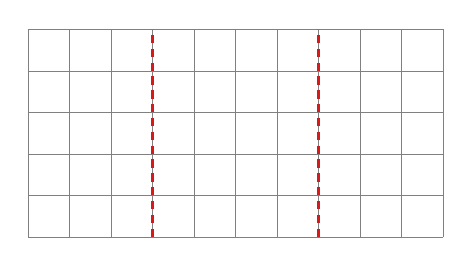
\begin{tikzpicture}[x=1.5em,y=1.5em]

  \draw[step=1, gray, very thin] (0,0) grid (10, 5);

  \drawstencil{3}{2}

  \onslide<2> {
    \draw[printred, densely dashed, very thick] (3,0) -- (3,5);
    \draw[printred, densely dashed, very thick] (7,0) -- (7,5);
  }
\end{tikzpicture}
\end{document}

    \end{figure}
  \end{frame}

  \begin{frame}
    \frametitle{Stencil Codes - \only<1>{Decomposition}\only<2->{Boundary Exchanges}}
    \begin{figure}
      \centering
      \input{fig/decomposition}
    \end{figure}
  \end{frame}

  \begin{frame}
    \frametitle{Stencil Codes}
    \begin{itemize}
      \item<1->{Memory-Centric Approach}
        \begin{itemize}
          \item{Load Neighbor Values from Memory}
          \item{Perform Calculation}
          \item{Store Result}
        \end{itemize}
      \item<2->{Not FPGA Friendly}
        \begin{itemize}
          \item{Random Access Memory Requirements}
          \item{Bi-directional data movement}
        \end{itemize}
    \end{itemize}
  \end{frame}













  \begin{frame}
    \frametitle{Stencil Codes - Communication}
    \begin{figure}
      \centering
      \documentclass[beamer]{standalone}
\definecolor{printred}{RGB}{215,25,28}
\usepackage{tikz}
\usepackage{lmodern}
\begin{document}
\tikzstyle{proc} = [circle, draw=black, fill=lightgray]

%TODO - use matrix, chains
% http://tex.stackexchange.com/questions/42611/list-of-available-tikz-libraries-with-a-short-introduction/43038#43038
\begin{tikzpicture}[]
  \matrix[row sep=1cm, column sep=2cm] {
    \node (A1) [proc] {}; &  \node (B1) [proc] {}; &  \node (C1) [proc] {}; \\
    \node (A2) [proc] {}; &  \node (B2) [proc] {}; &  \node (C2) [proc] {}; \\
    \node (A3) [proc] {}; &  \node (B3) [proc] {}; &  \node (C3) [proc] {}; \\
  };
  \path<1,2>[->]
    % Timestep 1 to Timestep 2
    (A1) edge[thick, dashed] (A2) 
    (B1) edge [thick] (A2)

    (B1) edge[thick, dashed] (B2)
    (C1) edge [thick] (B2)

    (C1) edge [thick, dashed] (C2)

    % Timestep 2 to Timestep 3
    (A2) edge[thick, dashed] (A3) 
    (B2) edge [thick] (A3)

    (B2) edge[thick, dashed] (B3)
    (C2) edge [thick] (B3)

    (C2) edge [thick, dashed] (C3)
  ;
  \onslide<1> {
    \path[->]

      (A1) edge[thick]  (B2) % zoot
      (B1) edge [thick] (C2) % zoot
      (A2) edge[thick]  (B3) % zoot
      (B2) edge [thick] (C3) % zoot
    ;
  }
\end{tikzpicture}
\end{document}

    \end{figure}
  \end{frame}

  \ifdraft{\def \stencilradius{1}}{\def \stencilradius{6}}
  % https://www.sharelatex.com/blog/2013/08/27/tikz-series-pt1.html

\documentclass[beamer]{standalone}
\usepackage{lmodern}
\usepackage{tikz}
\usetikzlibrary{calc}
\def \stencilradius{6}
\begin{document}
\begin{frame}
  \frametitle{Stencil Codes - Dependency Propagation}
  \begin{figure}
    \centering
    \begin{tikzpicture}[x=1em,y=1em]
      \def \maxrow {16}
      \def \maxcol {16}
      \def \originx{8}
      \def \originy{8}
      
      \foreach \sr in {1,...,\stencilradius}
      {
        \foreach \layer in {\sr,...,1}
        {
          \foreach \r in {0,...,\maxrow}
          {
            \foreach \c in {0,...,\maxcol}
            {
              \pgfmathparse{int(abs(\r - \originx) + abs(\c - \originy))}
              \ifnum \pgfmathresult < \layer
              \pgfmathparse{(\sr - \layer) * 15}
                \fill<\sr>[black!\pgfmathresult!lightgray] (\r,\c) rectangle (\r+1,\c+1);
              \fi
            }
          }
        }
      }
      \draw[step=1, gray, very thin] (0,0) grid (\maxrow+1, \maxcol+1);
    \end{tikzpicture}
  \end{figure}
\end{frame}
\end{document}


  \begin{frame}
    \begin{itemize}
      \item{Similar to ``Efficient temporal blocking for stencil computations by multicore-aware wavefront
      parallelization''}
    \end{itemize}
  \end{frame}
\end{document}
